%%%%%%%%%%%%%%%%%%%%%%%%%%%%%%%%%%%%%%%%%%%%%%%%%%%%%%%%%%%%%%%%%%%%%%%%%
% This file is part of the LaTeX sources of the OMDoc 1.3 specifiation
% Copyright (c) 2006 Bernd Krieg-Brueckner, Achim Mahnke
% This work is licensed by the Creative Commons Share-Alike license
% see http://creativecommons.org/licenses/by-sa/2.5/ for details
\svnInfo $Id: mmiss.tex 8453 2009-08-04 09:58:26Z kohlhase $
\svnKeyword $HeadURL: https://svn.omdoc.org/repos/omdoc/branches/omdoc-1.3/doc/spec/projects/semrelations/mmiss.tex $
%%%%%%%%%%%%%%%%%%%%%%%%%%%%%%%%%%%%%%%%%%%%%%%%%%%%%%%%%%%%%%%%%%%%%%%%%

\section{Semantic Interrelation and Change Management}
\begin{project}{MMiSS}{http://www.mmiss.de}
\pauthors{Bernd Krieg-Br{\"u}ckner\and  Achim Mahnke}
\pinstitute{Computer Science, University of Bremen, Germany}
\end{project}
The corpus of electronically available mathematical knowledge increases rapidly.  Usually,
mathematical objects are embedded in and related to different kinds of documents like
articles, books, or lecture material, the domain of which can be different from
mathematics, e.g., engineering or computer science. Therefore, maintaining high-quality
mathematical knowledge becomes a non-trivial engineering task for teams of authors.

In this scenario, sharing\twin{document}{sharing} and reuse\twin{document}{reuse} is the
key to efficient development. Unfortunately, while there has been a large body of research
concerning the sharing and reuse of program developments, sharing and reuse of documents
has until now been mainly done by little more than cut and paste.  However, to ensure
sustainable development, i.e. continuous long-term usability of the contents, sharing and
reuse needs to be supported by tools and methods taking into account the semantic
structure of the document. In developing these methods and tools we can benefit from the
experience in {\atwin{formal}{software}{development}} and associated support tools.

We address this problem by providing a methodology to specify coherence and consistency of
documents by interrelation of semantic terms and structural entities, supported by a tool
for fine-grained {\twintoo{version}{control}} and {\twintoo{configuration}{management}}
including {\twintoo{change}{management}}. Semantic
interrelation\twin{semantic}{interrelation} explicates the meaning lying behind the
textual content, and relates the semantic concepts within and across documents by means of
an ontology. To allow change management, each document is structured in-the-small.  Each
document corresponds to a package, and packages may be structured in-the-large using
folders and import relations. The ideas and methods explained here have been developed in
the \MMISS{} project which aimed at the construction of a multi-media Internet-based
adaptive educational system (see \cite{MMISS-WADT03,SemInter-DELFI04,MMISS-TechReport04}).

\subsection{Semantic Interrelation Via Ontologies}

Ontologies\index{ontology} provide the means for establishing a semantic structure. An
ontology is a formal explicit description of concepts in a domain of discourse. The
{\MMISS\LaTeX} package for ontologies provides a set of easy-to-use macros for the
declaration of ontologies in {\LaTeX} documents. They are used to {\emph{declare}} the
ontology of semantic terms used in a document, in a prelude up front. This
{\emph{specification}} of the document contains at least a rigorous hierarchical structure
of the terminology (a taxonomy, the {\emph{signature}} of the document), and may be seen
as an elaborate index structure. Moreover, relations between terms may be defined for more
semantic interrelation.

The ontology serves a dual purpose --- just as the specification of an
{\atwintoo{abstract}{data}{type}} in program development: it specifies the content to be
expected in the body of the document in an abstract, yet precise, manner --- the content
developers {\twintoo{requirement}{specification}}; and it specifies the content for
reference from the outside --- the user's perspective, who may then view the body of the
document as a black box. The content developer will use the {\MMISS\LaTeX} {\snippet{Def}}
command to specify the {\emph{defining}} occurrence of a promised term, as for an
index. Using the {\twintoo{structuring}{in-the-large}} facilities via packages, the
external user may then refer between documents using various kinds of {\emph{reference}}
commands, as the content developer may within a document.


  \begin{figure}[t]
    \begin{minipage}[b]{.6\textwidth}
      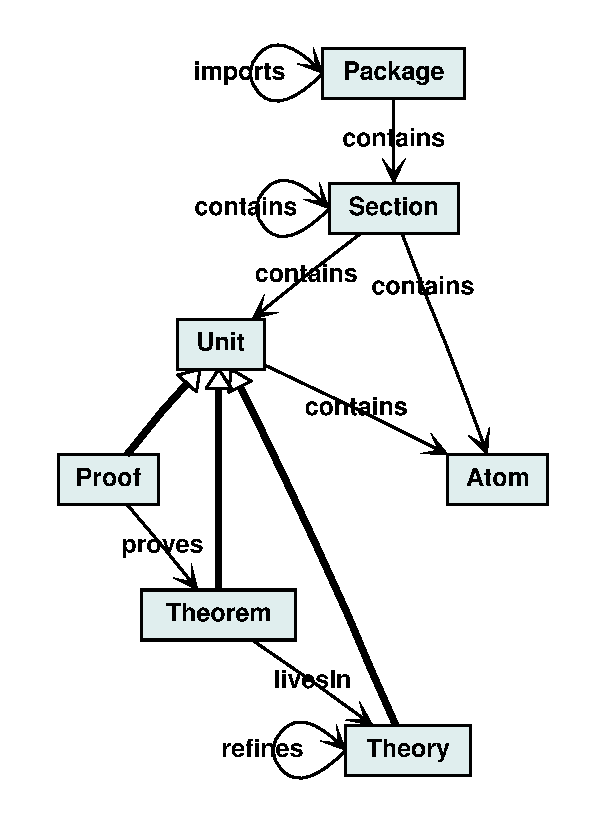
\includegraphics[width=.5\textwidth]{projects/semrelations/systems_onto_short}
    \end{minipage}
    \hspace*{-1cm}
    \begin{minipage}[b]{.4\textwidth}
      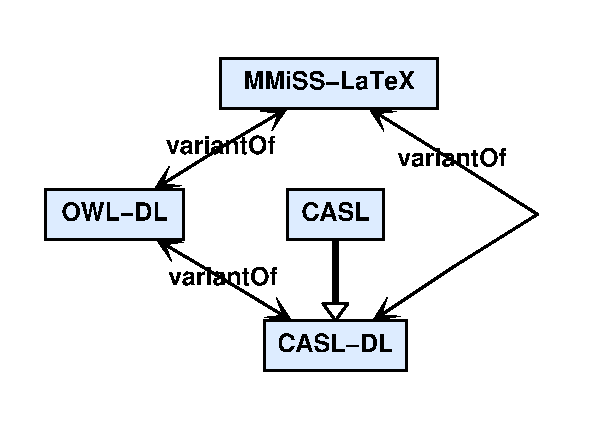
\includegraphics[width=1.1\textwidth]{projects/semrelations/onto_formalisms}
  \end{minipage}
  \caption{(a) Parts of the System's Ontology (b) Formalism variants}\label{fig:semrel-systems_onto}
\end{figure}

The next section will show, how we can explore this domain ontology --- supplied by the
author --- in order to capture semantic relations between document parts and use these
relations for supporting a management of change for mathematical documents.

\subsection{Change Management}

The notion of \emph{change management} is used for the maintenance and preservation of
consistency and completeness of a development during its evolution.  More precisely, we
want to have a {\twintoo{consistent}{configuration}} in which all versions are compatible
and there are no cyclic definitions or proofs.  At the same time, it should be a
{\twintoo{complete}{configuration}}: there should be no dangling forward references.

Such notions are well-known for formal languages. In contrast, natural language used for
writing teaching material does not usually possess a well-defined semantics, and the
notion of consistency is arguable.  Different authors may postulate different requirements
on the material in order to regard it as being consistent.  The existence of a
user-defined ontology helps a great deal to check references. However, we can make even
better use of the information contained in the ontology.

\paragraph{The System's Ontology}

The aim is to allow change management with regard to consistency and completeness
requirements defined by the user in terms of an ontology. In order to unify this approach
with the structural consistency and completeness properties introduced above, we express
the {\twintoo{document}{structure}}, originally defined by a document type definition, as
an ontology, the so-called \emph{System's Ontology} (see
Fig.~\ref{fig:semrel-systems_onto}a).  It defines the following relations between
structural elements of documents:
\begin{description}
\item [{\snippet{comprises}}] An obvious structuring mechanism is nesting of individual
  parts of a document, leading to the contains relation. The contains relation is part of
  a family of {\snippet{comprises}} relations that share common properties.
\item [{\snippet{reliesOn}}] A family of {\snippet{reliesOn}} relations reflects the
  various dependencies between different parts of a document.  For example, a theorem
  \emph{lives in} a theory, or proof \emph{proves} a theorem.
\item [{\snippet{pointsTo}}] The family of {\snippet{pointsTo}} relations is very similar,
  and relates references with the defining occurrence of a semantic term.
\item [{\snippet{variantOf}}] Another structuring relation is introduced by
  variants. Parts of a document may e.g. be written in various languages which gives rise
  to a {\snippet{variantOf}} relation between these document parts and their constituents;
  it is an equivalence relation.
\end{description}

It is now rather straightforward to formulate consistency and completeness rules in terms
of invariants of these relations. Formulating these invariants as formal rules will enable
us to implement a generic and flexible {\twintoo{change}{management}} that keeps track of
the invariants and informs the user about violations when a previously consistent document
has been revised, leading to various kinds of error (e.g. for {\snippet{reliesOn}}
relations) or warning messages (e.g. for {\snippet{pointsTo}} relations).


\paragraph{Properties of Interactions between Structuring Mechanisms.}
This approach also allows us to lift relations to structuring mechanisms allowing more
modular and localized change management.  For example, relating the {\snippet{comprises}}
and {\snippet{reliesOn}} relations allows us to formalize invariants regarding the closure
of document parts with respect to the {\snippet{reliesOn}} relation: We can require that
there is a proof for each theorem in a package.  Furthermore, if two structural entities
are related by {\snippet{reliesOn}}, their relation is propagated along the
{\snippet{comprises}} relation towards the root of the hierarchy of nested structural
entities, such that (for a theorem $T$ a proof $P$, and sections $A, B$):

\begin{description}
\item[] $B$ contains $P$ \& $A$ contains $T$ \& $P$ proves $T \Rightarrow B$
  {\snippet{reliesOn}} $A$.
\end{description}

% \[\text{B contains P and A contains T and P proves T, then
%         B reliesOn A.}
% \]

If the user changes section $A$, the repository will only need to check all sections that
$A$ relies on (such as $B$ here) for invariants, and not the whole document. However, in
contrast to formal developments as in e.g. the MAYA system \cite{AH-05-a}, there is no
rigorous requirement that a document should obey all the rules.  There may be good
reasons, for instance, to present first a "light-weight" introduction to all notions
introduced in a section before giving the detailed definitions. In this particular case,
one would want to introduce forward pointers to the definitions rather than making the
definitions rely on the introduction; thus the rules are covered.

In any case, the more structure there is, the better the chances are for preserving
consistency and completeness; any investment in introducing more {\snippet{reliesOn}}
relations, for example, will pay off eventually. The change management will observe
whether revisions by the user will affect these relations and, depending on the user's
preferences, emit corresponding warnings.

The aim is to allow users to specify individual notions of consistency by formulating the
rules that the relations should obey. This should be possible for the relations between
the particular (predefined) structuring mechanisms, but also in general between semantic
terms of the user's own ontology. Our work in this direction will rely on the methods and
tools provided by the {\hets} system (see {\mysecref{hets}}).

\subsection{Variants}

The concept of {\indextoo{variant}s} adds a new dimension to hierarchically
{\twintoo{structured}{document}s}.  The idea is to maintain and manage different variants
of structural entities (document subtrees) which represent the same information in
different ways --- variants are meant to glue them together.

Managing different natural language variants in parallel is an obvious example.  Another
one is the formalism variant which denotes the particular formalism in which a formal
content part like a theorem or a definition is expressed. Considering ontology development
itself, for example, we propose to use variants to maintain different formal
representations for the same semantic concept together with its documentation.
Figure~\ref{fig:semrel-systems_onto}b shows the possible variants for declaring ontology
components (see \cite{WOSE-2004} for details).

The \MMISS{} repository provides functions to store and retrieve these structural variants
by means of specifications for selecting particular variants for editing or presentation.

\subsection{Relations to {\omdoc}}

{\omdoc} provides modules for marking up the knowledge structure and the narrative
structure of mathematical documents. \MMISS{} combines these two viewpoints by giving
means for structuring the document contents (which constitutes the narrative structure) and
for specifying the incorporated knowledge by use of ontologies. Therefore, we have
implemented an export of \MMISS{} documents to (content and narrative) {\omdoc} documents
and vice versa.

% LocalWords:  MMiSS Bernd Krieg ckner Achim Mahnke multi reliesOn pointsTo
% LocalWords:  variantOf hets subtrees versa
